\section{\framework{}: a framework for virtual exocentric vision systems}
\label{sec:rear}
In this section we will describe \framework{} - 
\textit{Rear Exocentric Augmented Reality}, a framework 
for the development of virtual exocentric vision systems.
%
It has been written in C++, following an object-oriented 
approach, and implements the minimal set of tools and functionalities 
needed to create representations of a mobile robot in its environment 
through the use of augmented reality techniques, as described in 
section \ref{sec:exo}.
%

%
For what concerns graphics, \framework{} relies on OpenGL.
It makes use of three software components: a \textit{camera}, 
a 3D model of the \textit{robot} itself and a \textit{texture}.
%
The camera provides the user with a view of the OpenGL space 
from a certain point-of-view and with a certain field-of-view. 
It identifies a \textit{viewing frustum} - as shown in figure 
\ref{fig:openglspace} - whose volume corresponds to the 
portion of OpenGL space displayed on the user's screen.
%
To give the user the illusion of seeing the robot from an 
external point-of-view, the 3d model of the robot is drawn 
within the viewing frustum, while the more distant frustum base 
is applied a texture displaying a picture previously 
captured from the robot's egocentric camera.
%

%
An example of what a user sees is showed in figure \ref{fig:snap}.
%
\begin{figure}[!h]
  \begin{center}
    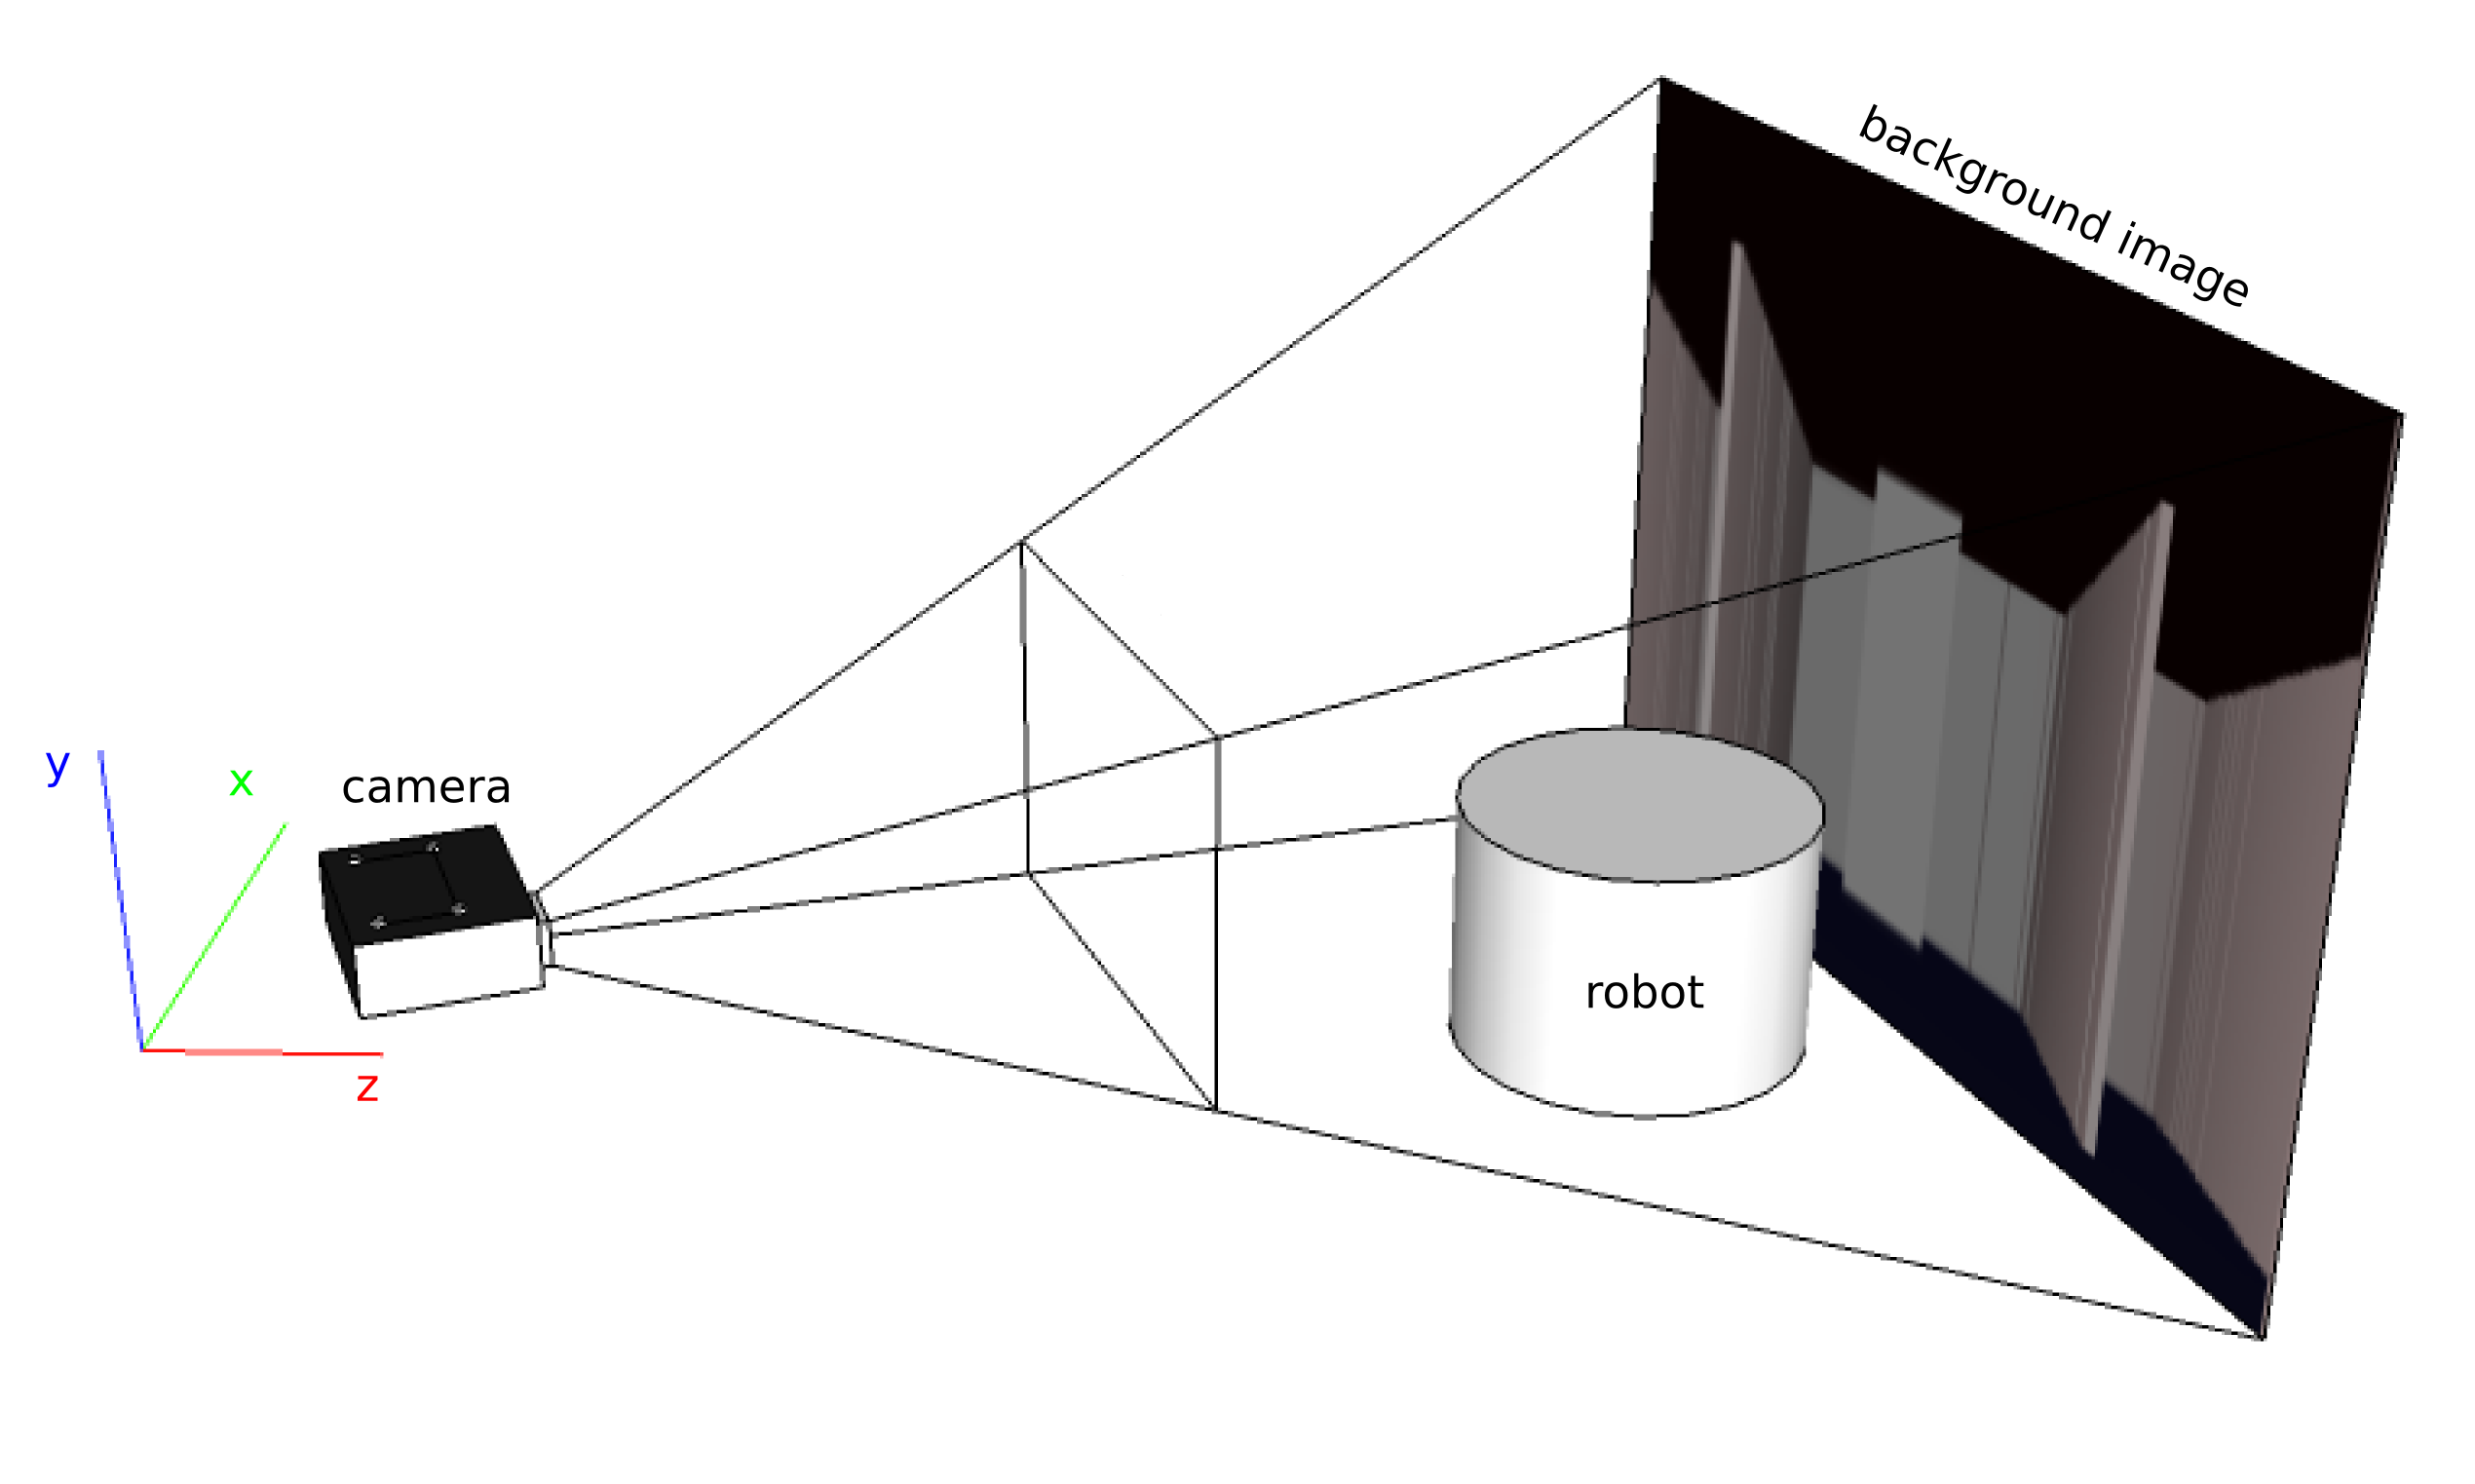
\includegraphics[width=300pt]{img/camera_frustum_scheme.png}
    \caption{The OpenGL space}
    \label{fig:openglspace}
  \end{center}
\end{figure}
%
\begin{figure}[!h]
  \begin{center}
    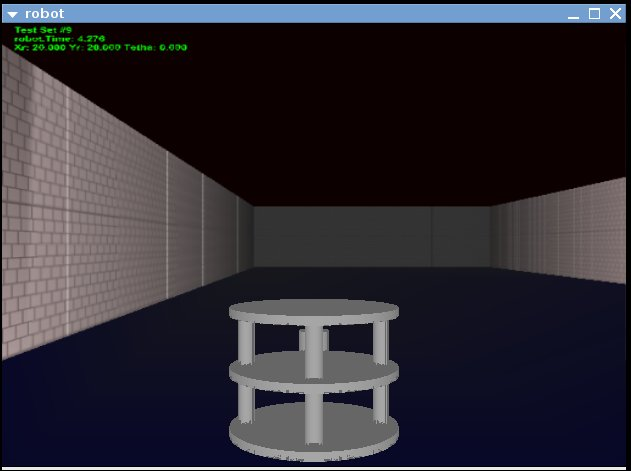
\includegraphics[width=300pt]{img/rear_snapshot_large.jpg}
    \caption{A snapshot from a \framework{}-based application}
    \label{fig:snap}
  \end{center}
\end{figure}
%

%
Main issues in the approach we have just described are 1. 
\textit{where} to draw the robot within the viewing frustum 
and 2. \textit{which} of the captured images is to be used 
as background.
%
For what concerns the first issue, one can intuitively guess 
that the simplest way to determine the robot position 
within the frustum is to know the current robot position 
and orientation and the position and orientation of the egocentric 
camera when the snapshot was taken and, then, to set the 
position of the 3d model of the robot and the point-of-view 
of the camera accordingly.
Well, that's what \framework{} does.
%
Therefore, to run, every \framework{} concrete implementation 
needs, at least:
%
\begin{itemize}
  \item a set of snapshots captured from the robot egocentric camera, 
    together with the robot position at the time it was taken
  \item the robot's current position
\end{itemize}
%
Such data is retrieved every time the operator, using the 
interface provided by \framework{} itself, sends a 
motion command to the robot.
%
After collecting new data, which include new robot status and
the associated egocentric camera image, \framework{} chooses 
an image to set as background and draw the robot model within 
the frustum. So, for what concerns issue no. 2, as already 
underlined in \cite{sugimoto}, let us say that there is not 
a \textit{unique} way to determine which image is to be set 
as background, since different image selection algorithms 
would differently affect user perceptions and. We will have a 
deeper look at some image selection algorithms in section
\ref{sub:iimageselector}.
%
Finally, the overall execution loop is resumed by the flowchart 
showed in figure \ref{fig:overall_diagram}.
%
\begin{figure}[!h]
  \begin{center}
    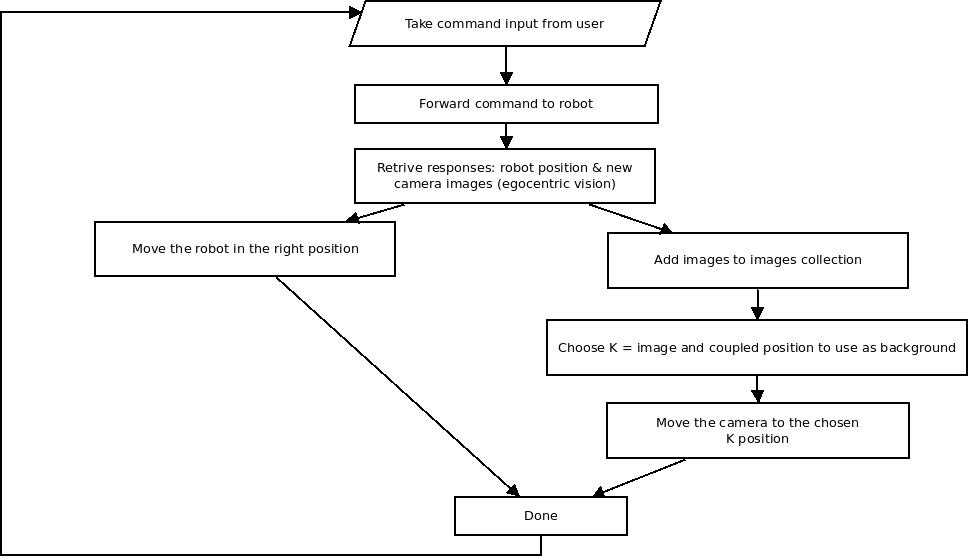
\includegraphics[width=400pt]{img/overall_diagram.jpeg}  %robot pic
    \caption{Application flowchart}
    \label{fig:overall_diagram}
  \end{center}
\end{figure}

\subsection{Class diagram}
\label{sec:classdiagram}
%
Let us have a look at \framework{} class diagram, 
showed in figure \ref {fig:class_diagram}.
%
\begin{figure}[!h]
  \begin{center}
    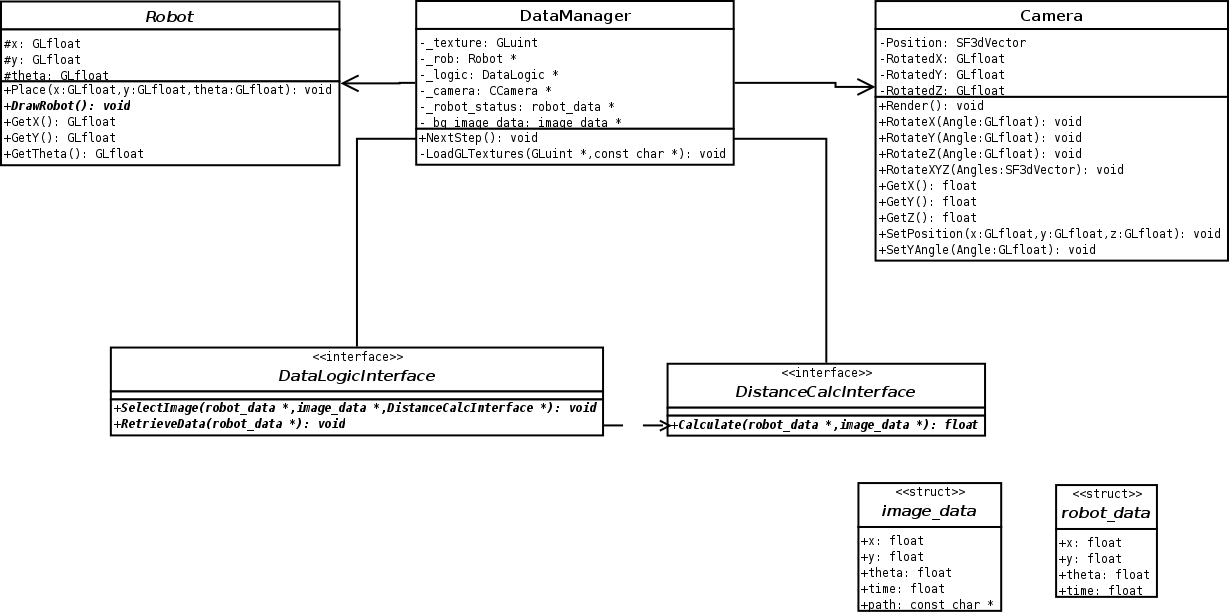
\includegraphics[width=400pt]{img/rear_class_diagram.png}
    \caption{\framework{} class diagram}
    \label{fig:class_diagram}
  \end{center}
\end{figure}
%
Two of the components needed by \framework{}, the robot 
model and the camera, are mapped on two dedicated classes, 
\texttt{Robot} and \texttt{Camera}, respectively.
%

%
The former is an \textit{abstract class}, serves as a storage 
for the current position and orientation of the actual
robot and declare a pure virtual method in which subclasses 
must include all of the procedure to draw the OpenGL model 
of the robot itself.
%
The latter is instead a \textit{helper class}, since there 
exists no actual camera within the OpenGL space. The camera 
model is just an abstraction used to give a more intuitive
way to set the portion of space the user is looking at.
In fact, the \texttt{Camera} class provides methods to 
set the user's point-of-view within the OpenGL space (see
chapter \ref{sec:cameraclass}).
%

%
In the middle, between \texttt{Robot} and \texttt{Camera},
there is the \texttt{DataManager} class. It is intended to be 
the core of every \framework{} based application, since it 
internally implements the loop showed in figure 
\ref{fig:overall_diagram}.
It acts as a \textit{mediator} among all of the other classes, 
in that it manages their interaction and, hence, reduces 
coupling between them.
%

%
The diagram also features two interfaces that have to be implemented 
by programmers who want to create their own concrete exocentric 
vision system: \texttt{IDataLogic} and 
\texttt{IImageSelector}.
%

%
The former decouples the application 
core, that is the \texttt{DataManager}, from the data source.
This way, \texttt{DataManager} code can be totally unaware of 
the technology used to retrieve data from the robot - e.g. 
sockets, web services, etc.
%

%
\texttt{IImageSelector}, instead, defines the interface 
of the component which implements the image selection algorithm.
%
In this case, the use of an interface leaves programmers 
able to change, and even to implement new image 
selection algorithms without having to worry about
changing other classes.
%

%
Finally, the class diagram presents two structures, 
\texttt{image\_data} and \texttt{robot\_data}, whose 
declarations are reported in listing \ref{code:data}.
%
The former is used to store all the metadata 
relative to a specific snapshot - i.e. the position 
and the orientation of the camera when it was taken, 
a timestamp and an array of chars that can be used by 
programmers who would like to add other data - e.g. 
a code or a sequence number.
%

%
The latter is similar to the former, it is meant to be 
used by \texttt{DataManager} to exchange information
about the current robot position and orientation with 
lower-level objects, in a compact way.
%
\begin{lstlisting}[caption={\framework{} data structures}, label={code:data}, frame=trBL]
struct image_data {
  float x;
  float y;
  float theta;
  float time;
  char path[100];
};

struct robot_data {
  float x;
  float y;
  float theta;
  float time;
};
\end{lstlisting}
%

%
In the following of this section, we will have a look 
\textit{under the hood} of the classes and interfaces 
we have just introduced.
%
We will see how \framework{} functionalities are 
mapped onto them and, then, how to correctly subclass/use
them in order to build a concrete exocentric vision system.
%

%
\subsubsection{The Robot Class}
\label{sub:robotclass}
Let us have a look at the declaration of the \texttt{Robot}
class, reported in listing \ref{code:robot_class}.
%
\begin{lstlisting}[caption={\texttt{Robot} class declaration}, label={code:robot_class}, frame=trBL]
class Robot
{
 private:
  GLfloat x;
  GLfloat y;					
  GLfloat theta;

 public:
  Robot();
  GLfloat GetX();
  GLfloat GetY();
  GLfloat GetTheta();
  void Place(GLfloat x, GLfloat y, GLfloat theta);
  virtual void DrawRobot() = 0;
};
\end{lstlisting}
%
As already stated, private attributes of \texttt{Robot} 
are used to store the current position and orientation 
of the actual robot. Such attributes are initialized with 
all-zeros by the constructor, can be read by means 
of invoking their \textit{getter} methods and can be set 
by means of the \texttt{Place()} method.
%

%
\texttt{Robot} also declares an abstract \textit{hook} method, 
\texttt{DrawRobot()}. Such a method is called by the 
\texttt{DataManager} every time it wants to render the 
robot model and, hence, programmers who wants to 
use \framework{} for their own robot should subclass 
\texttt{Robot} and implement \texttt{DrawRobot()} as a 
procedure that draws their custom robot model using 
the OpenGL API.
%
When doing that, one must always keep in mind that 
\framework{} makes use of a three-dimensional OpenGL 
space, while position information is often represented 
as a \texttt{(x,y)} pair. \texttt{R.E.A.R.} maps the \texttt{x} 
value of such a pair onto the x axis of its OpenGL space, 
while the \texttt{y} value is mapped onto the z axis.
%
That is, the actual XY plan corresponds to the OpenGL 
XZ plan. Such a correspondence is represented in figure 
\ref{fig:reference_systems}.
%
\begin{figure}[!h]
  \begin{center}
    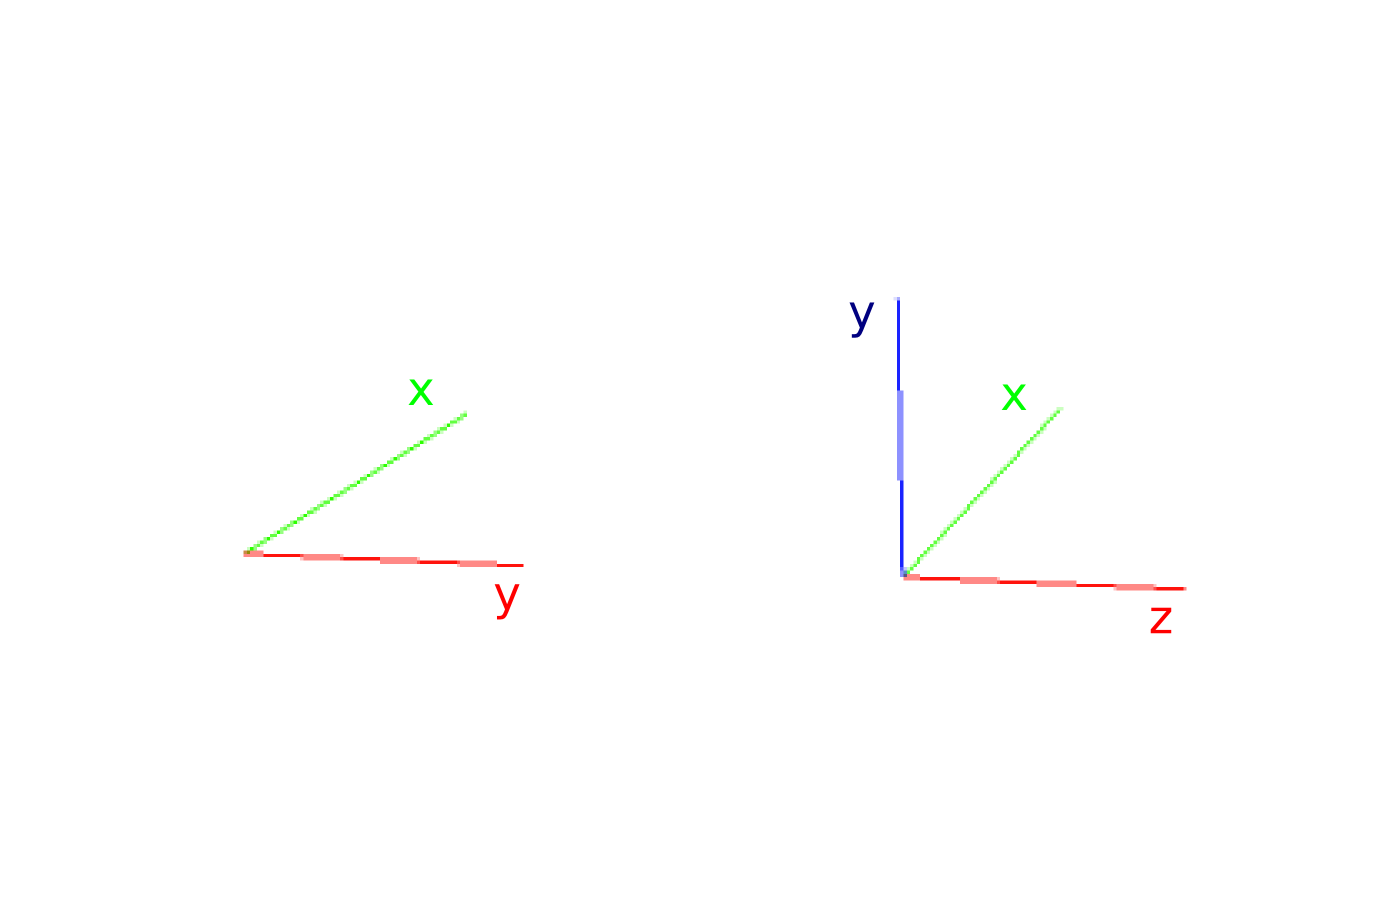
\includegraphics[width=300pt]{img/reference_system.png}
    \caption{Reference systems}
    \label{fig:reference_systems}
  \end{center}
\end{figure}
%

%
Moreover, to draw the robot in the right position within 
the OpenGL space, the first thing a \texttt{DrawRobot()} should 
do is to invoke OpenGL function \texttt{glTranslate()}.
%

%
A skeleton of a concrete implementation of \texttt{DrawRobot()}
would look like this:
\begin{lstlisting}[caption={\texttt{DrawRobot()} skeleton}, label={code:drawrobot_skeleton}, frame=trBL]  
  glMatrixMode(GL_MODELVIEW);
  glPushMatrix();

  // set robot position
  glTranslatef(this -> x, 0.0f, this -> y);

  // rotate the robot 
  glRotatef(this -> theta, 0.0f, 1.0f, 0.0f);

  // code to actually draw the robot

  glPopMatrix();
\end{lstlisting}
%

%
\subsubsection{The Camera Class}
\label{sub:cameraclass}

OpenGL does not provide any \textit{camera}, anyway it proved 
to be extremely useful to have a helper class that permits 
to easily set position and orientation of the user's 
point of view and sight, without worrying about lower-level 
OpenGL details.
%

%
A basic implementation of such a helper class is suggested 
in \cite{opengl:camera}. Such an implementation is slightly 
similar the one featured by \framework{}, whose 
declaration is reported in listing \ref{code:camera_class}.
%
\begin{lstlisting}[caption={\texttt{Camera} class declaration}, label={code:camera_class}, frame=trBL]
class Camera
{
 private:
  SF3dVector Position;
  GLfloat RotatedX, RotatedY, RotatedZ;	
  GLfloat _theta;

 public:
  Camera();
  void Render ( void );
  void Move ( SF3dVector Direction );
  GLfloat GetX();
  GLfloat GetY();
  GLfloat GetZ();
  GLfloat GetTheta();
  void SetPosition(GLfloat x, GLfloat y, GLfloat z);
  void SetYAngle ( GLfloat Angle );
  void RotateX ( GLfloat Angle );
  void RotateY ( GLfloat Angle );
  void RotateZ ( GLfloat Angle );
  void RotateXYZ ( SF3dVector Angles );
};
\end{lstlisting}
%
The \texttt{Camera} class allows to move and rotate the user 
point of view, independently from the robot.
%
This is essential for our purposes, since \framework{}
must be able to draw the robot everywhere in the OpenGL space, 
regardless of where the camera is, and vice versa.
%

%
\texttt{Camera} methods are pretty simple: they just make 
use of OpenGL basic commands (such as \texttt{glTranslate} 
and \texttt{glRotate}) to actually move the OpenGL reference 
system and, hence, move the point-of-view and change the sight 
direction.
%
The only thing to care about when using such a class is 
to invoke the OpenGL commands \texttt{glMatrixMode(GL\_MODELVIEW)} 
and \texttt{glLoadIdentity()} before invoking its 
\texttt{Render()} method. This avoids previous modifications 
of the \texttt{GL\_MODELVIEW} matrix from affecting the 
positioning of the camera.
%

%
\subsubsection{The DataManager Class}
\label{sub:datamanager}

As already stated, the \texttt{DataManager} class is the \textit{core}
of the whole framework. Its declaration is reported in 
listing \ref{code:datamanager_class}.
%
\begin{lstlisting}[caption={\texttt{DataManager} class declaration}, label={code:datamanager_class}, frame=trBL]
class DataManager
{
 private:
  GLuint _texture[1];
  Robot * _rob;
  Camera * _camera;
  IDataLogic * _logic;
  IImageSelector * _calculator;

  robot_data * _robot_status;
  image_data * _bg_image_data;

  /* bind the specified image to a texture */
  void LoadGLTextures(GLuint *, const char *);

 public:
  DataManager(Robot *, DataLogic *, Camera *, 
	      IImageSelector *); 
  ~DataManager();
  void NextStep(int command = 0);
};
\end{lstlisting}
%
Of course, \texttt{DataManger} is meant to be used as a \textit{singleton}, 
that is, there must be a unique instance of \texttt{DataManager} 
within the context of a \framework{} based application.
%
As its name suggests, \texttt{DataManager} manages and coordinates 
all of the components of the exocentric vision system and, hence, 
keeps a private reference to all of them: 
the \texttt{Robot} instance (see section \ref{sub:robotclass}), the 
\texttt{Camera} instance (see section \ref{sub:cameraclass}),
a \texttt{IDataLogic} object, a \texttt{IImageSelector} 
object and an OpenGL texture id number.
%

%
Once the application is started, it's \texttt{DataManger}'s duty 
to move robot and camera within the OpenGL space. Moreover, 
it's also responsible for 1. providing the user an interface 
to send commands to the robot, 2. retrieving position 
data from the actual robot every time the user asks 
for it, 3. for picking one of the available snapshots, 
4. displaying it in the background. 
%
All of these operations are performed within the 
scope of \texttt{NextStep()} method, reported in 
listing \ref{code:next_step}.
%
\begin{lstlisting}[caption={The \texttt{DataManager::NextStep()} method}, label={code:next_step}, frame=trBL]
void DataManager::NextStep(int command) {

  image_data old_image;

  // save metadata of the currently displayed 
  // image
  old_image.x = _bg_image_data -> x;
  old_image.y = _bg_image_data -> y;
  old_image.theta = _bg_image_data -> theta;


  // send command to the robot
  _logic->Command(command);

  // retrieve new data from the robot
  _logic->RetrieveData(_robot_status);

  // move robot with _robot_status data
  _rob->Place(_robot_status->x,
	      _robot_status->y,
	      _robot_status->theta ); 

  // choose an image to set as background
  _logic->SelectImage(_robot_status, _bg_image_data,
		      _calculator);

  // if the chosen image is not the currently
  // displayed one, then  move the camera
  // into the new position and change its 
  // orientation accorgindly
  if ( old_image.x != _bg_image_data -> x ||
       old_image.y != _bg_image_data -> y ||
       old_image.theta != _bg_image_data -> theta )
    {
      _camera -> SetPosition( _bg_image_data -> x,
			      0.f,
			      _bg_image_data -> y);
      
      _camera -> SetYAngle( _bg_image_data -> theta - 90);
    }

  // actually set the chosen image as background
  LoadGLTextures(_texture, _bg_image_data->path);
}
\end{lstlisting}
%
\texttt{NextStep()} has to be called every time 
the user wants to send a command to the robot. 
%
Such a command, encoded as an integer, has to be passed to 
\texttt{NextStep()} as an argument.
%
Then, \texttt{DataManager} asks its \texttt{IDataLogic} 
instance to send the command to the robot and to 
retrieve the new robot position and orientation, which will be 
stored in the \texttt{\_robot\_status} private attribute.
%

%
To select an image to set as background, \texttt{DataManager} 
invokes the \\
\texttt{IDataLogic::SelectImage()} method, 
passing it the current robot position and orientation, 
an object of type \texttt{IImageSelector} which 
encapsulates the image selection algorithm and a structure 
of type \texttt{image\_data}.
%
The method will fill the fields of such a structure with 
the metadata of the selected image, so that the 
\texttt{DataManager()} can pick it up, load it as a 
texture and display it on the background of the 
viewing frustum - by means of calling the 
\texttt{LoadGLTextures()} function.
%

%
In order to give the illusion of watching the scene 
from the point the selected image was taken, 
\texttt{NextStep()} also moves the camera and change 
its orientation accordingly to the image metadata.
%

\subsubsection{The IDataLogic interface}
\label{sub:idatalogic}

\texttt{IDataLogic} provides a communication interface 
with the robot, decoupling the \texttt{DataManager} 
from the actual technology used to interact with it 
and to collect data from it. Its declaration is: 
\begin{lstlisting}[caption={\texttt{IDataLogic} declaration}, label={code:idatalogic}, frame=trBL]
class IDataLogic {
 public:
  virtual void Command(int) = 0;
  virtual void RetrieveData(robot_data *) = 0;
  virtual void SelectImage(robot_data *, image_data *,
			   IImageSelector *) = 0;
};
\end{lstlisting}
%
When implementing a class of type \texttt{IDataLogic}
programmers should keep in mind the followings:
\begin{itemize}
  \item \texttt{RetrieveData()} must fill the passed 
    robot\_data structure with the retrieved position and
    orientation of the robot. It must also keep track of 
    all retrieved snapshots.
  \item \texttt{SelectImage()} is passed the robot's current 
    position and orientation and an object of type 
    \texttt{IImageSelector}. In order to obtain the image 
    to set as background (whose metadata will be saved 
    in the \texttt{image\_data} structure), an 
    invocation of the \texttt{IImageSelector::ChooseImage()}
    is required (for further details, see chapter
    \ref{sub:iimageselector}).
\end{itemize}
%
A skeleton of either \texttt{RetrieveData()} and 
\texttt{SelectImage()} is presented in listing 
\ref{code:idatalogic_skeleton}.
%
\begin{lstlisting}[caption={\texttt{IDataLogic} methods skeleton}, label={code:idatalogic_skeleton}, frame=trBL]
void DataLogic::RetrieveData( robot_data * data )
{
  // actually retrieve new data

  // store the collected snapshot into an
  // internal data structure
  
  data -> x = retrieved_robot_data.x;
  data -> y = retrieved_robot_data.y;
  data -> theta = retrieved_robot_data.theta; 
  data -> time = retrieved_robot_data.time;

  return;
}

void DataLogic::SelectImage( robot_data * robot_status, 
                             image_data * bg_image_data,
			     IImageSelector * calculator )
{
  // say we have used a vector to store 
  // metadata of the collected snapshots, 
  // then we could invoke the ChooseImage method

  selector -> ChooseImage( robot_status, bg_image_data, 
                             &_images_collection );
}
\end{lstlisting}
%

%
\subsubsection{The IImageSelector interface}
\label{sub:iimageselector}

Last, but not least, the \texttt{IImageSelector} interface
defines the type of classes that encapsulate an image 
selection algorithm. It declares just a method, that 
we have already encountered in the previous section:
%
\begin{lstlisting}[caption={\texttt{IImageSelector} declaration}, label={code:iimageselector}, frame=trBL]
class IImageSelector
{
 public:
  virtual void ChooseImage(robot_data *, image_data *, 
                           std::vector<image_data> *) = 0;
};
\end{lstlisting}
%
\texttt{ChooseImage()} is passed the current robot position and
orientation and a vector of images metadata. It will process them 
and will fill the passed \texttt{image\_data} structured fields 
with the metadata of the selected image.
%

%
Say we want to define a class that implements the selection 
method 2 presented in \cite{sugimoto}. That selection method
chooses the image taken as near as possible to the robot
current position.
%

%
The \texttt{Calculate()} function, called within the following code,
estimates the euclidean distance between robot and a generic image.
If we decided to choose the closest image to the robot, we would
show the egocentric vision, because the algorithm would always
select the image coupled with distance equal to zero. We remember
that the egocentric vision image is always present in our images' set.
%
In order to not show only the egocentric vision, the \texttt{ChooseImage()}
does not return the image coupled with the minimum distance, but the one
(if available) with the minimum distance greater than zero.
%

We could, then, write:
\begin{lstlisting}[caption={A possible \texttt{ChooseImage} implementation}, label={code:chooseimage_impl}, frame=trBL]
class SpacialMetricSelector : public IImageSelector
{
  public:
  void ChooseImage(robot_data *, image_data *, 
                   std::vector<image_data> *);
};


void SpacialMetricSelector::
      ChooseImage( robot_data * robot_status, 
                   image_data * bg_image_data,
		   std::vector<image_data> * 
                      _images_collection)
{

  float distances[_images_collection->size()];
  float min;

  // calculate the distance for each stored image
  int i = 0;
  for (std::vector<image_data>::iterator it =
	 _images_collection->begin();
       it != _images_collection->end();
       it++)
    {
      distances[i] = Calculate(robot_status, &*it);
      i++;
    }

  // find the minimum distance
  i = 0;
  min = distances[0];
  for (int j = 1; j < _images_collection->size(); j++)
    {
      if ( ( distances[j] < min && min != 0) || 
           ( distances[j] > min && min == 0)    )
	{
	  i = j;
	  min = distances[j];
	}
    }

  // return the selected image data
  bg_image_data->x = (*_images_collection)[i].x;
  bg_image_data->y = (*_images_collection)[i].y;
  bg_image_data->theta = (*_images_collection)[i].theta;
  bg_image_data->time = (*_images_collection)[i].time;
}
\end{lstlisting}
%
